% nicht reguläre Sprache
Über dem Alphabet $\Sigma=\{\texttt{0},\texttt{1}\}$ ist die Sprache
\[
L
=
\{
w\in\Sigma^*
\mid
|w|_{\texttt{0}}
-
|w|_{\texttt{1}}
\in
\{1,2\}
\}
\]
gegeben.
Ist $L$ regulär?

\begin{loesung}
\definecolor{darkred}{rgb}{0.8,0,0}
\definecolor{darkgreen}{rgb}{0,0.6,0}
Die Sprache ist nicht regulär, wie man mit dem Pumping Lemma für reguläre
Sprachen beweisen kann:
\begin{enumerate}
\item Annahme: $L$ ist regular.
\item Nach dem Pumping Lemma gibt es die Pumping Length $N$
\item Wähle das Wort $w = \texttt{0}^{N+1}\texttt{1}^N$
\begin{center}
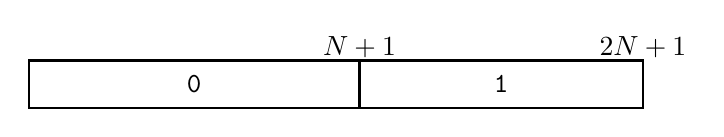
\begin{tikzpicture}[>=latex,thick]
\def\h{0.6}
\draw (0,0) rectangle ({13*\h},\h);
\draw ({7*\h},0) -- ++(0,\h);
\node at ({3.5*\h},{0.5*\h}) {\texttt{0}};
\node at ({10*\h},{0.5*\h}) {\texttt{1}};
\node at ({7*\h},{\h-0.1}) [above] {$N+1$};
\node at ({13*\h},{\h-0.1}) [above] {$2N+1$};
\end{tikzpicture}
\end{center}
\item Nach dem Pumping Lemma gibt es eine Aufteilung
$w={\color{darkgreen}x}{\color{darkred}y}{\color{blue}z}$
mit
$|
{\color{darkgreen}x}
{\color{darkred}y}|\le N$ und
$|{\color{darkred}y}|> 0$.
\begin{center}
\begin{tikzpicture}[>=latex,thick]
\def\h{0.6}
\draw (0,0) rectangle ({13*\h},\h);
\draw ({7*\h},0) -- ++(0,\h);
\node at ({3.5*\h},{0.5*\h}) {\texttt{0}};
\node at ({10*\h},{0.5*\h}) {\texttt{1}};
\node at ({7*\h},{\h-0.1}) [above] {$N+1$};
\node at ({13*\h},{\h-0.1}) [above] {$2N+1$};
\fill[color=darkgreen!20,opacity=0.7]
	(0.05,0.05) rectangle ({3*\h-0.025},{\h-0.05});
\draw[color=darkgreen]
	(0.05,0.05) rectangle ({3*\h-0.025},{\h-0.05});
\node[color=darkgreen] at ({1.5*\h},{0.5*\h}) {$x\mathstrut$};
\fill[color=darkred!20,opacity=0.7]
	({3*\h+0.025},0.05) rectangle ({6*\h-0.025},{\h-0.05});
\draw[color=darkred]
	({3*\h+0.025},0.05) rectangle ({6*\h-0.025},{\h-0.05});
\node[color=darkred] at ({4.5*\h},{0.5*\h}) {$y\mathstrut$};
\fill[color=blue!20,opacity=0.7]
	({6*\h+0.025},0.05) rectangle ({13*\h-0.05},{\h-0.05});
\draw[color=blue]
	({6*\h+0.025},0.05) rectangle ({13*\h-0.05},{\h-0.05});
\node[color=blue] at ({9.5*\h},{0.5*\h}) {$z\mathstrut$};
\end{tikzpicture}
\end{center}
\item
Es folgt, dass der Teil
${\color{darkred}y}$
nur aus Nullen besteht.
Durch Aufpumpen kann die Zahl $|w|_{\texttt{0}}$ beliebig
vergrössert werden, während $|w|_{\texttt{1}}$ gleich bleibt.
Damit wird auch $|w|_{\texttt{0}} - |w|_{\texttt{1}}$ beliebig gross
und damit ist ein solches gepumptes Wort nicht mehr in $L$, im 
Widerspruch zur Aussage des Pumping Lemma.
\item
Dieser Widerspruch zeigt, dass $L$ nicht regulär ist.
\qedhere
\end{enumerate}
\end{loesung}

\begin{bewertung}
6 Schritte des Pumping-Lemma-Beweises:
Annahme ({\bf A}) 1 Punkt,
Pumping Length ({\bf N}) 1 Punkt,
Wort ({\bf W}) 1 Punkt,
Unterteilung ({\bf U}) 1 Punkt,
Widerspruch beim Pumpen ({\bf P}) 1 Punkt,
Folgerung ({\bf F}) 1 Punkt.
\end{bewertung}

